\subsection{Pedido de ventas con transporte propio}

%!!! cambiar esto por el diagrama de visio cuando este :)
\subsubsection{Cursograma}
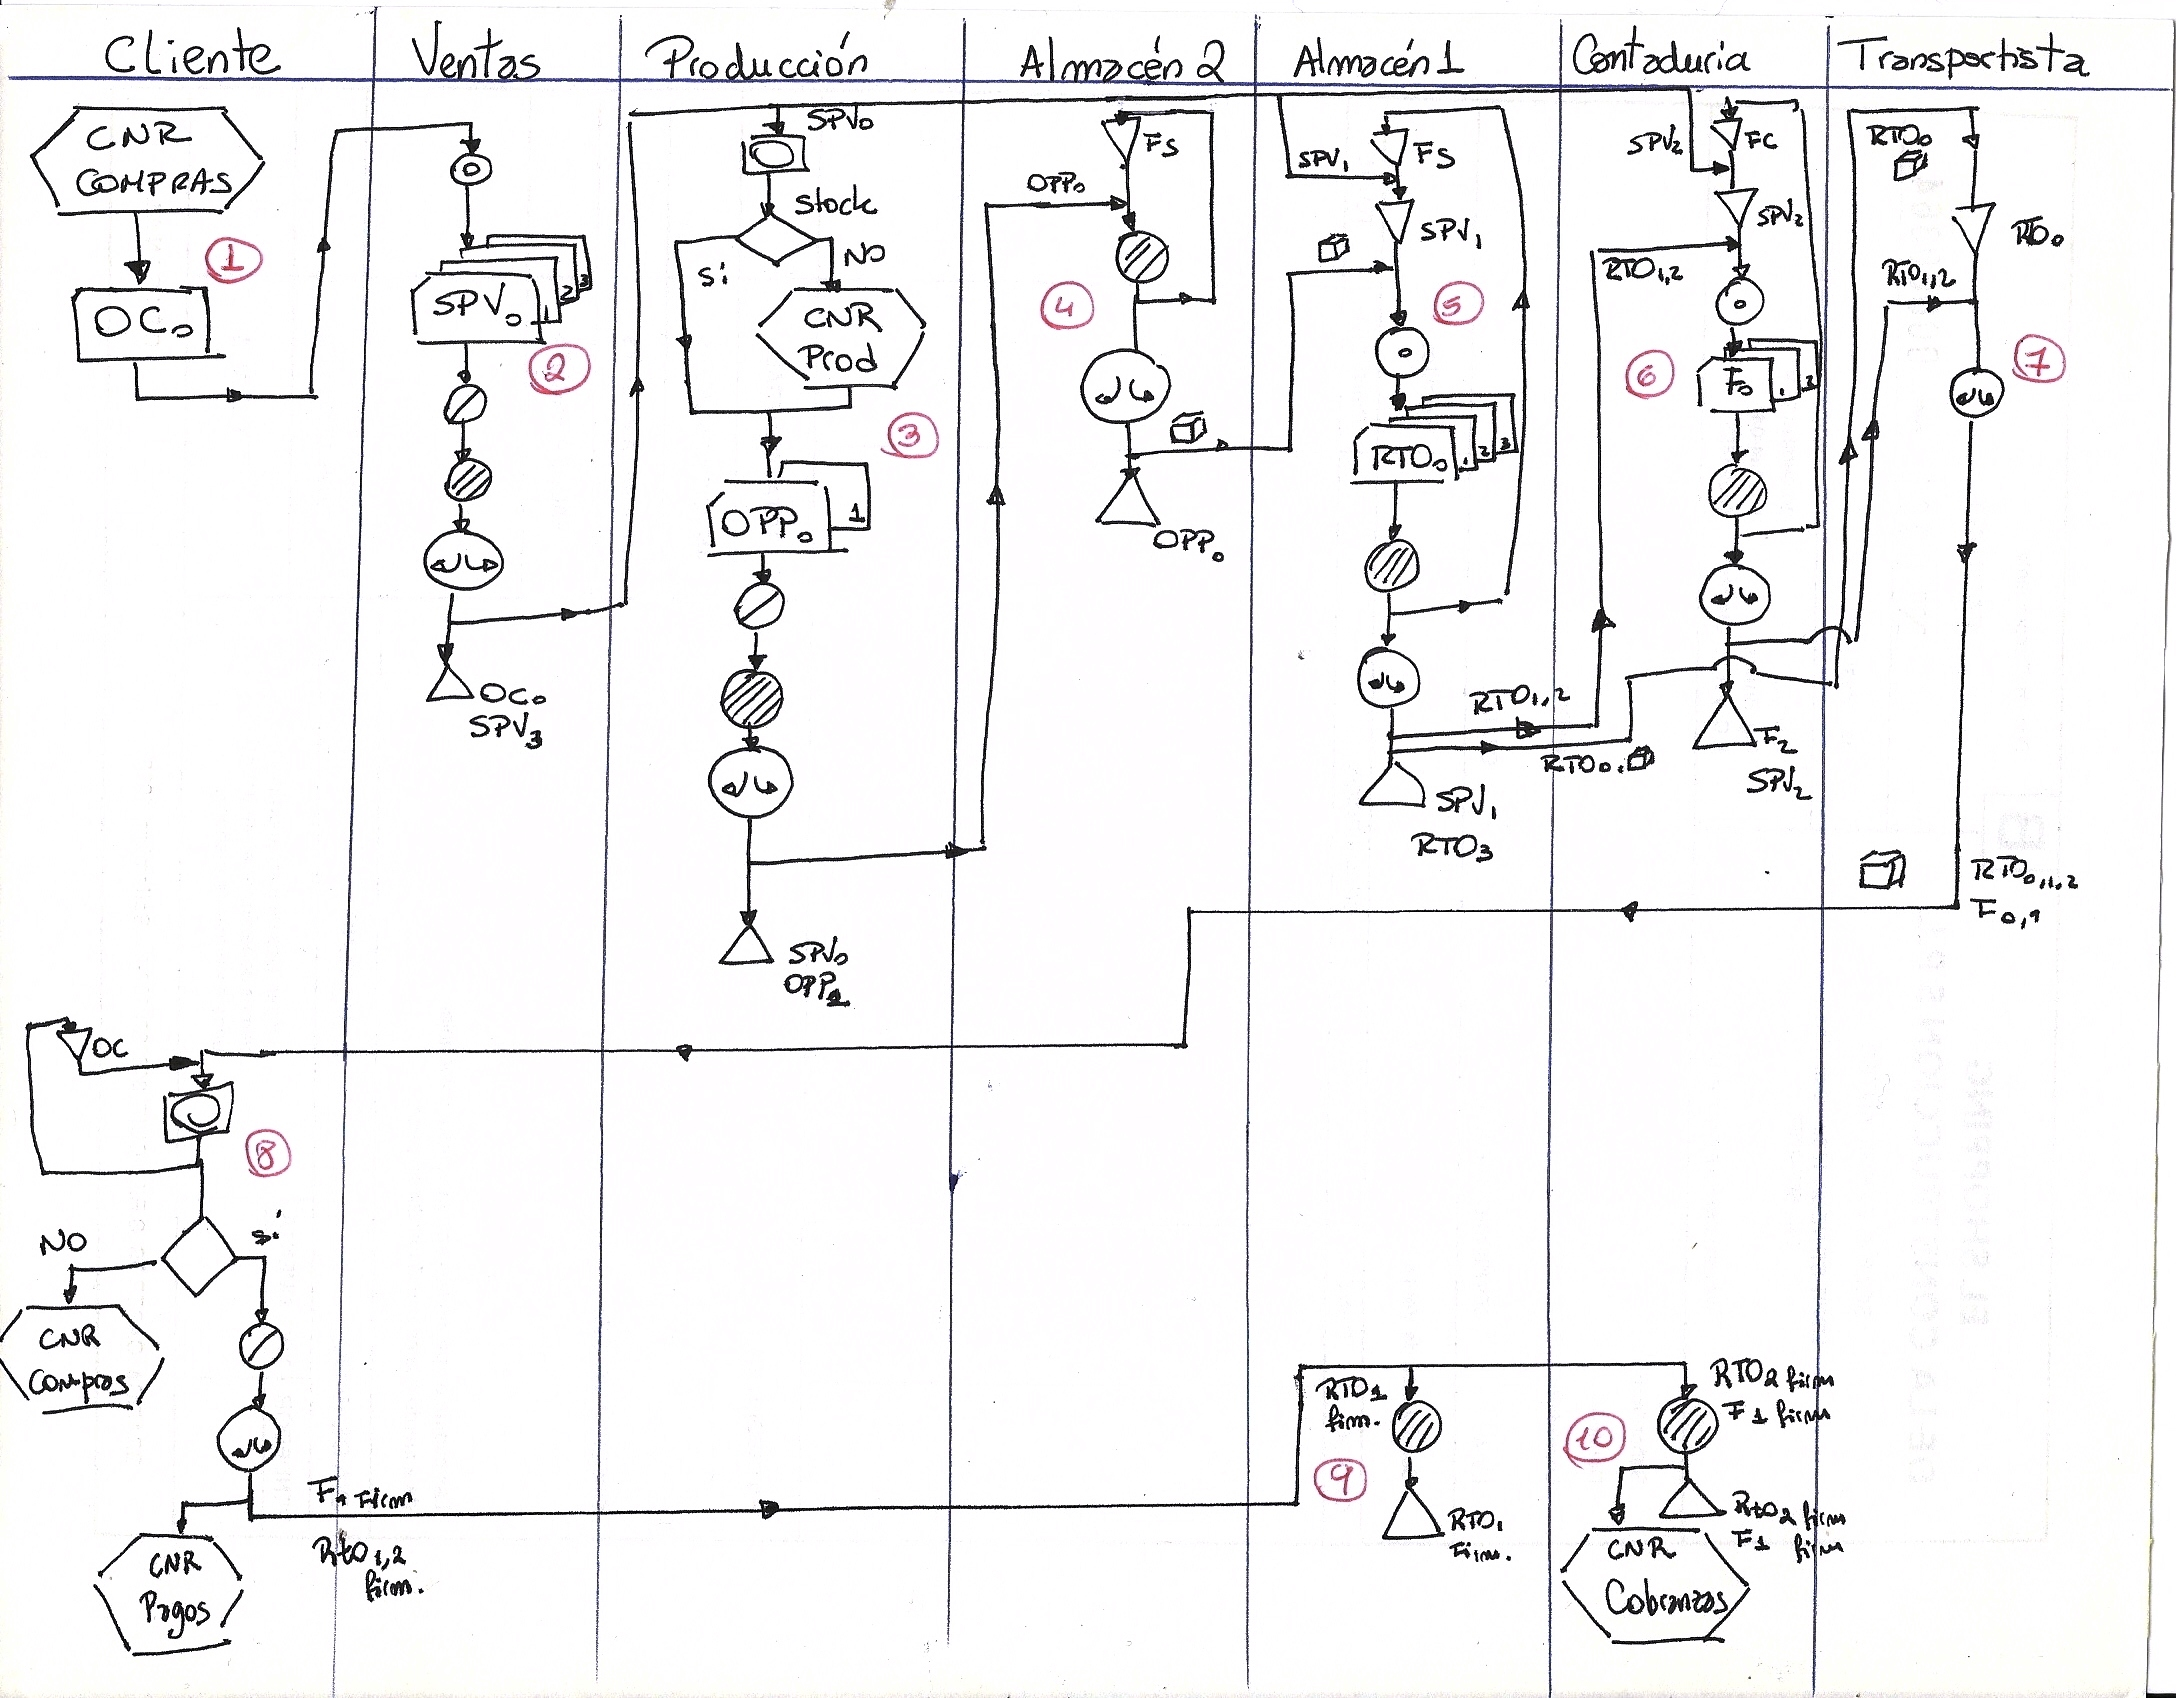
\includegraphics [angle=90]{Empresa/Circuitos/Ventas/ventas.jpg}

\pagebreak

\subsubsection{Procedimiento}
\begin{enumerate}
\item El cliente solicita un pedido
\item Ventas genera la Solicitud de Pedido de Ventas (SPV) especificando los detalles de la venta (productos, plazo de entrega tentativo).
	Firma la SPV y envia una copia a Producci\'on. Archiva temporalmente esta solicitud hasta que concluya el pedido.
\item Producci\'on recibe la SPV y verifica que cuenta con stock. De no poseer stock necesario se procede a realizar el CNR de Producci\'on. 
	En caso de contar con el producto solicitado, se envia ``una orden de pedido de productos'' a Almac\'en 2 ( almacén de productos terminados ).
\item Almac\'en 2 recibe la orden de producto ( ya cuenta con el producto, ya sea porque ten\'ia stock o porque lo ha producido especialmente ) y lo env\'ia al  Almac\'en 1 ( Expedici\'on).
\item Almac\'en 1 prepara los productos para su entrega y genera el remito correspondiente, con 2 copias. Entrega el producto al Transportista con los remitos original y copia para que sean firmados por el cliente y env\'ia otra copia a Contadur\'ia.
\item Contadur\'ia genera un listado de remitos sin facturar asociados a esa SPV, y genera la factura correspondiente. Se envia el original de la factura al Transportista para su env\'io.
\item Transportista recibe original y copia del remito y la factura. Env\'ia el pedido junto con la documentaci\'on al cliente.El cliente recibe el original de la factura y del remito, y firma la copia del remito.
\item Almacen 1 recibe la copia del remito firmado por el cliente y cierra la orden de pedido. 
\item Contadur\'ia recibe la copia de la factura y el remito firmado por el cliente y la asienta como recibida por el cliente. El pago de la factura es parte del CNR de Cobros.Contaduria
\end{enumerate}

\subsubsection{Entrevista}

Luego de analizar los diagramas de procedimiento de alto nivel del proceso de ventas que la empresa puso a nuestra disposici\'on, surgi\'o la necesidad de realizar una entrevista para aclarar ciertos puntos que no quedaban claros con nuestro contacto. Los puntos en cuesti\'on fueron los siguientes:

\begin{description}
 \item \underline{Ventas a Clientes}: \\
	Es el Centro de Atenci\'ion al Cliente (\textit{CAC}) quien interact\'ua con los clientes para realizar las ventas. Las ventas a clientes las ventas se realizan a partir de un pedido de cotizaci\'on confeccionado por el CAC. Posteriormente, el CAC formaliza el pedido de venta al recibir una Orden de Compra del cliente. Internamente, el CAC realiza una Solicitud de Pedido de Ventas (SPV).  \\
	Para el caso de los Distribuidores, ellos reciben la lista de precios y pueden formalizar directamente la Orden de Compra, es decir, que no hay cotizaci\'on previa del CAC.
 \item \underline{Registro de Clientes}: \\
	La empresa mantiene un registro de los clientes, y las transacciones que realizan con la empresa, mediante el sistema ERP Bejerman. Esta base de datos es actualizada por el \'area de Ventas, a trav\'es del \textit{CAC} y es consultada por todas las personas de la empresa que tienen habilitada esa funci\'on dentro de los m\'odulos del sistema inform\'atico. 
 \item \underline{Moviemiento de Materiales}: \\
	El medio de comunicaci\'on entre almacenes es electr\'onico, es decir, se realiza a trav\'es del sistema Bejerman, y as\'i se realizan las transferencias ``inter-dep\'osito''. Los documentos internos s\'olo se imprimen en papel cuando resulta necesario, y en casos particulares. En una \'epoca se utilizaban fichas y vale de materiales, pero fueron reemplazados por el sistema inform\'atico. Lo mismo sucede con el sector de Producci\'on, que maneja el movimiento de materiales mediante el sistema Bejerman.\\
	El sector de Producci\'on recibe por sistema la carga de datos del \'area de Ventas (CAC), formaliz\'andolo como ``Orden de Pedido''. En funci\'on a ello elabora una ``Orden de Montaje'', donde el sistema carga los elementos necesarios para confeccionar el pedido solicitado (las distintas partes y piezas para armar la luminaria). Terminado el producto, \'este se declara en el Dep\'osito Producto Terminado (02). Luego, el sector de Almacenes realiza por sistema la transferencia del producto, desde el 02 al Deposito Principal (01), y es desde aqu\'i que el \'area de Expedici\'on puede generar posteriormente el remito para despachar la mercader\'ia.  
	El transportista carga la mercader\'ia seg\'un la información emanada de los remitos, controlando f\'isicamente la carga.  Luego se le confecciona una Hoja de Ruta con el itinerario diario y por ultimo se le emite un permiso ante el ARBA, en caso que la mercader\'ia que se transporte supere los \$20.000.-   
	
\end{description}

\subsubsection{Normas de Control Interno}
\begin{itemize}
 \item	{\bf Separaci\'on de funciones: } El encargado de ventas no debe poseer acceso a las registraciones de stock ni a la modificaci\'on de cuentas del cliente.
Quien vende no puede otorgar cr\'editos ni encargarse de la facturaci\'on. Dentro del sector de Ventas existe una clara divisi\'on entre la parte encargada de la atenci\'on a los clientes 
y la parte encargada de la venta en s\'i misma.
\item	{\bf Aprobaci\'on de la venta: } Las pol\'iticas de ventas, otorgamiento de cr\'editos y precios son dispuestas por la Direcci\'on General.
La aprobaci\'on de la venta es realizada por el responsable de cr\'editos dado que es el que conoce el estado financiero de los clientes.
\item	{\bf Movimiento de bienes: } La circulaci\'on de mercader\'ias est\'a respaldada por comprobantes firmados por el responsable del sector que los recibe. En los sectores de Producci\'on, 
Almac\'en 1 y 2 y Expedici\'on se documenta el transpaso de mercader\'ia utilizando el correspondiente m\'odulo del sistema inform\'atico de Bejerman.
\item	{\bf Documentaci\'on prenumerada: } Toda documantaci\'on emitida debe estar prenumerada y se archivan en orden num\'erico, incluso las anuladas. Dado que todos los documentos se generan 
utilizando el sistema inform\'atico, resulta complicado alterar la numeraci\'on dado que la misma es autogenerada utilizando una secuencia.
\item	{\bf Control de Facturaci\'on: } Contadur\'ia realiza un control cruzado de la facturaci\'on y remitos. Contadur\'ia siempre conserva una copia de las facturas y remitos emitidos. 
A su vez, realiza un control antes de que dichos documentos sean enviados al cliente.
  

\end{itemize}



\pagebreak

\subsubsection{Formularios de Ventas}

\paragraph{\underline{Factura}}
\begin{flushleft}
  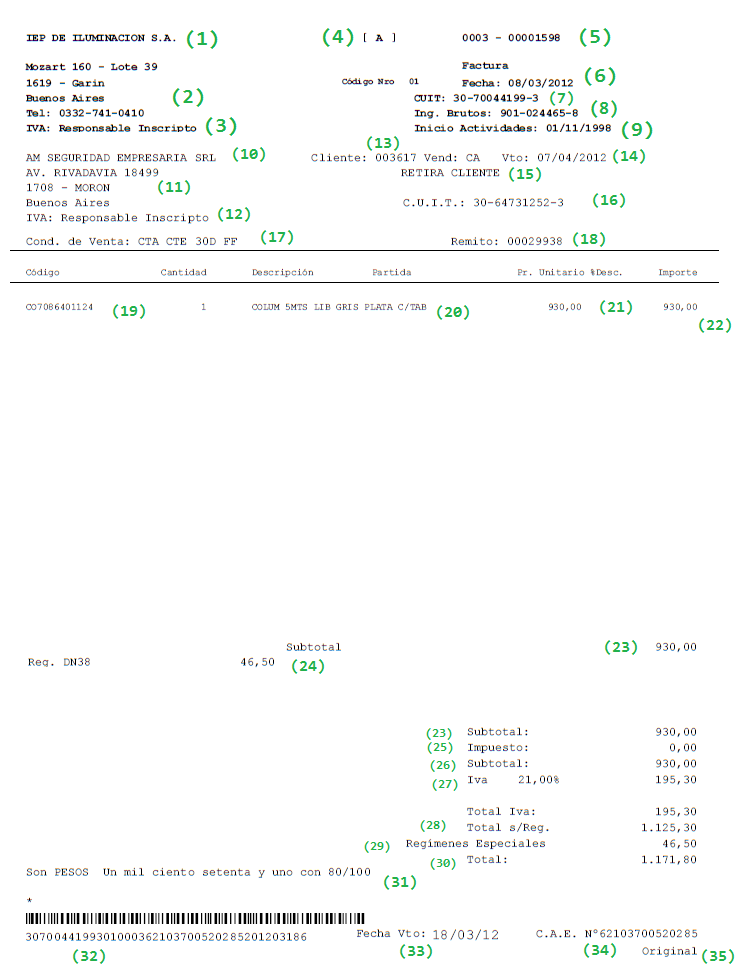
\includegraphics[scale=0.85]{./Images/FormulariosIEP/Factura.png}\end{flushleft}
  \begin{itemize}
	  \item \textbf{Objetivo:} Con este documento se notifica al cliente que efectu\'o la compra el monto total a pagar. Se especifica el remito asociado, los productos comprados con detalle de precios, los impuestos incluidos y las condiciones de pago.
	  \item \textbf{Alcance:} Es un documento entre la empresa y el cliente.
	  \item \textbf{Emisor:} Contadur\'ia.
	  \item \textbf{Cantidad de Copias Emitidas:} Original y Copia.
	  \item \textbf{Sector receptor:} Expedici\'on, para su env\'io al cliente.
	  \item \textbf{Descripci\'on de Campos de la factura}
  \end{itemize}

  \begin{enumerate}
   \item Empresa emisora: Raz\'on Social de la empresa
   \item Empresa emisora: Información de Sucursal. Domicilio y N\'umero de Tel\'efono
   \item Empresa emisora: Responsabilidad frente al IVA
   \item Tipo de Factura (A en este caso)
   \item N\'umero de Factura
   \item Fecha de emisi\'on
   \item Empresa emisora: CUIT
   \item Empresa emisora: C\'odigo de Ingresos Brutos
   \item Empresa emisora: Fecha de inicio de actividades
   \item Cliente: Raz\'on Social 
   \item Cliente: Domicilio
   \item Cliente: Responsabilidad frente al IVA
   \item C\'odigo del cliente al que se le factura y C\'odigo de Vendedor (Opcional)
   \item Vencimiento de la Factura
   \item Condici\'on de entrega
   \item Cliente: CUIT
   \item Condici\'on de Venta / Tipo de Pago.
   \item Remito asociado a la Venta.
   \item Detalle de la factura: C\'odigo interno del \'item, Cantidad del \'item
   \item Detalle de la factura: Descripci\'on del \'item. La partida asociada es opcional
   \item Detalle de la factura: Precio unitario del \'item. El descuento del \'item es opcional.
   \item Detalle de la factura: Precio total del \'item (cantidad * precio unitario)
   \item Detalle de la factura: Subtotal de items (suma de los totales de \'item)
   \item Detalle de la factura: Detalle de Regímenes Especiales que aplican.
   \item Total de Impuestos que aplican a la venta (sin IVA).
   \item Subtotal con Impuestos y sin IVA.
   \item IVA discriminado.
   \item Subtotal con Impuestos e IVA, sin Reg\'imenes Especiales.
   \item Total de Reg\'imenes Especiales.
   \item Total del Importe de la Factura.
   \item Importe de la factura en palabras.(Opcional)
   \item C\'odigo de Barras de la factura. El c\'odigo tambi\'en se encuentra en forma num\'erica. 
   \item Fecha de vencimiento del C\'odigo de Impresi\'on
   \item CAE: C\'odigo de Autorizaci\'on Electr\'onico.
   \item Copia de la facura: Original, Copia, Triplicado, etc
      
  \end{enumerate}

\paragraph{\underline{Remito}}
 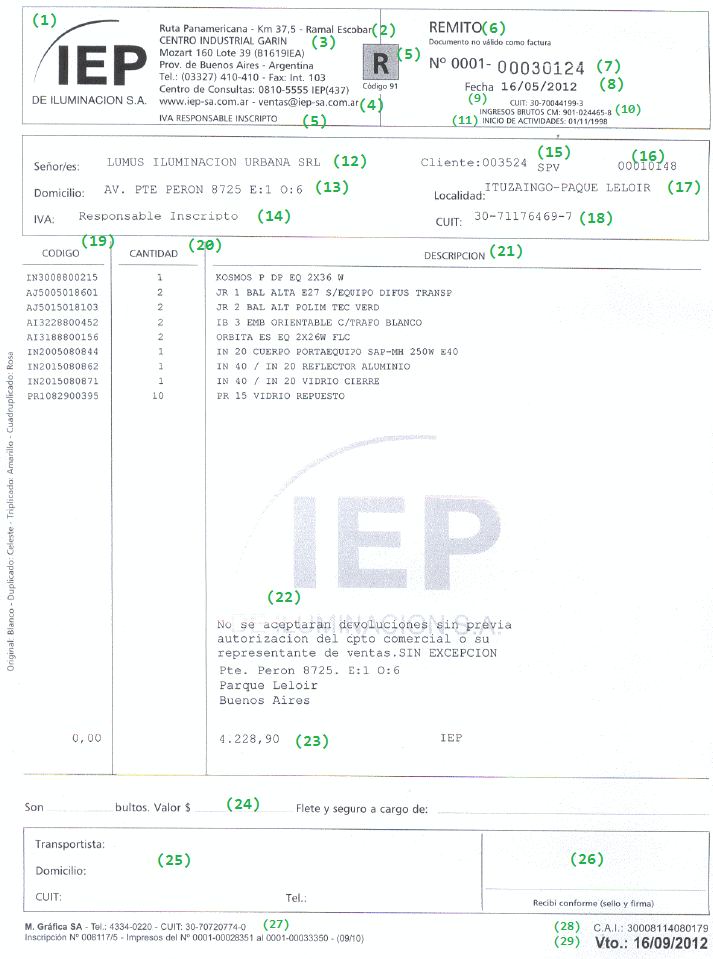
\includegraphics{./Images/FormulariosIEP/Remito.png}
 \begin{itemize}
	  \item \textbf{Objetivo:} En este documento se detallan los productos a ser enviados al cliente. No se incluyen detalles de precios y se especifica la contidad de bultos.
	  \item \textbf{Alcance:} Es un documento entre la empresa y el cliente.
	  \item \textbf{Emisor:} Almacén 1.
	  \item \textbf{Cantidad de Copias Emitidas:} Original y Copia.
	  \item \textbf{Sector receptor:} Expedición, para su envío al cliente.
 \end{itemize}




